\section{SYSTEM OVERVIEW}
\subsection{Problem Formulation}
%refine the stream and event pattern %
%define the pattern we deal formally%
% include base line 1 batch size in experemintal results%

We follow the terminology of \cite{luckham2008power,alevizos2015complex,zhou2015pattern} to formalize the problem we tackle. Given a set of \emph{$K$} real-time streams of events $S = \{ s_1,s_2, ..., s_k\}$ as input, which are associated with a set of $K$  objects $O = \{ o_1, ..., o_k\}$. Where each stream $s_i=\langle e_1,e_3,...,e_t,...\rangle$  is a time-ordered sequence of events, these events are connected to a moving object  $o_i \in O$,  $e_t$  refers to the current time event within the unbounded stream, we give the definition of the input event sample as follows:  
\begin{definition}
	Each event is defined as a tuple of attributes $$e_i = (type,\tau,a_1,a_2.....,a_n,id)$$ Where $type$ is the event type attribute that takes a value from a set of finite event types/symbols $\Sigma$, $\tau$ represents the timestamp of the event tuple,  the  $a_1,a_2,...,a_n$ are spatial or other contextual features (e.g., speed); these features are varying from one application domain to another, while the $id$ attribute connects the event tuple to an associated moving object.
\end{definition}

A user-defined pattern $\mathcal{P}$ is given in the form of regular expression over $\Sigma$ (i.e., event types) \cite{alevizos2017event}, and the main goal is to predict the full matches of $\mathcal{P}$ within each event stream $s_i\in S$ in real-time.

\par The setting that is considered in this work is described in the following:\\
A large-scale patterns prediction over multiple input event streams system that  consists of $K=\left\vert{S}\right\vert$ distributed predictor nodes $n_1,n_2...,n_k$, each of which consumes an input event stream $s_i\in S$, and provides an online predication service. Each node $i \in [K]$ handles a single event stream $s_i$ associated with a moving object $o_i \in O$, in addition,  it  maintains a local prediction model $f_i$ for the user-defined pattern $\mathcal{P}$. An online prediction about the future full match of the pattern $\mathcal{P}$ in $s_i$ is provided for each new arriving event tuple. In summary, we have multiple running instances of an online prediction algorithm on distributed nodes for multiple input event streams, each instance provides online predications about a pre-defined pattern of events.  We consider as input a massive event streams that describe trajectories of  moving objects, more specifically, event streams of moving vessels in the context of maritime surveillance.  

The defined pattern $\mathcal{P}$ is monitored over each event stream $s_i$  by a  predictor nodes  $n_i$  that maintains a local prediction model $f_i$, where there is one node for each vessel's event stream.  The prediction model $f_i$ gives the ability to provide an online predictions about when the pattern will be completed in the form of an expected number of future events before a full match does occur.

\subsection{The Proposed Approach}
\label{sec:proposed_approach}
\par We design and develop a scalable and distributed patterns prediction system over massive input event streams of moving objects. We  exploit the event forecasting with Pattern Markov Chains \cite{alevizos2017event} as the base prediction model (i.e., $f_i$).Moreover,  we propose to enable the information exchange between the distributed predictors/learners of the input event streams, by adapting the distributed online predication protocol \cite{dekel2012optimal,kamp2014communication} to synchronize the prediction models, i.e., Markov transitions probabilities of the Pattern Markov Chain (PMC) predictors.

\par We propose a $synchronization operation$  for the distributed Pattern Markov Chain (PMC) models based on the maximum-likelihood estimation \citep{anderson1957statistical} for the transition probabilities matrix of the underlaying Markov Chain described by: 
\begin{equation}
\label{eq:pi_estim}
\hat{p}_{i,j}=\frac{\sum_{k \in K} n_{k,i,j}}{\sum_{k \in K} \sum_{l \in L} n_{k,i,l}}
\end{equation}


\par Our approach relies on enabling the collaborative learning between the prediction models of  the input event streams. By doing so, we assume that the underlying event streams belong to the same  distribution and share the same behavior (e.g., mobility patterns). We claim that assumption is reasonable in many application domains, for instance, in the context of maritime surveillance, vessels travel through defined routes by International Maritime Organization (IMO). Additionally, vessels have similar mobility patterns in specific areas such as moving with low speed and multiple turns near the ports \cite{pallotta2013vessel,liu2014knowledge}. That allows our system to dynamically construct a coherent global prediction model for all input event streams based on merging its local models.

\par By enabling collaborative learning our approach is imposing an acceleration of learning of the underlying prediction models with less training data, in addition, it provides an improvement of the predictive performance compared to the no-distributed  version of event forecasting with Pattern Markov Chains system. 


\subsection{Distributed Architecture}
\label{sec:architecture}
Our system consumes an aggregated events stream as input\footnote{In practice, the aggregated input events stream is composed of multiple input event streams for multiple moving objects, which are reconstructed bt the system internally.} of large number of moving objects, which is continuously collected and fed into the system. It allows users to register a pattern $\mathcal{P}$ to be monitored over each event stream of a moving object. Output stream consists of original input events alongside with predictions of full matches of $\mathcal{P}$ is outputted to be displayed to the end users. Figure ~\ref{fig:architecture} presents the overview of our system architecture and its main components.      


\begin{figure}[h]

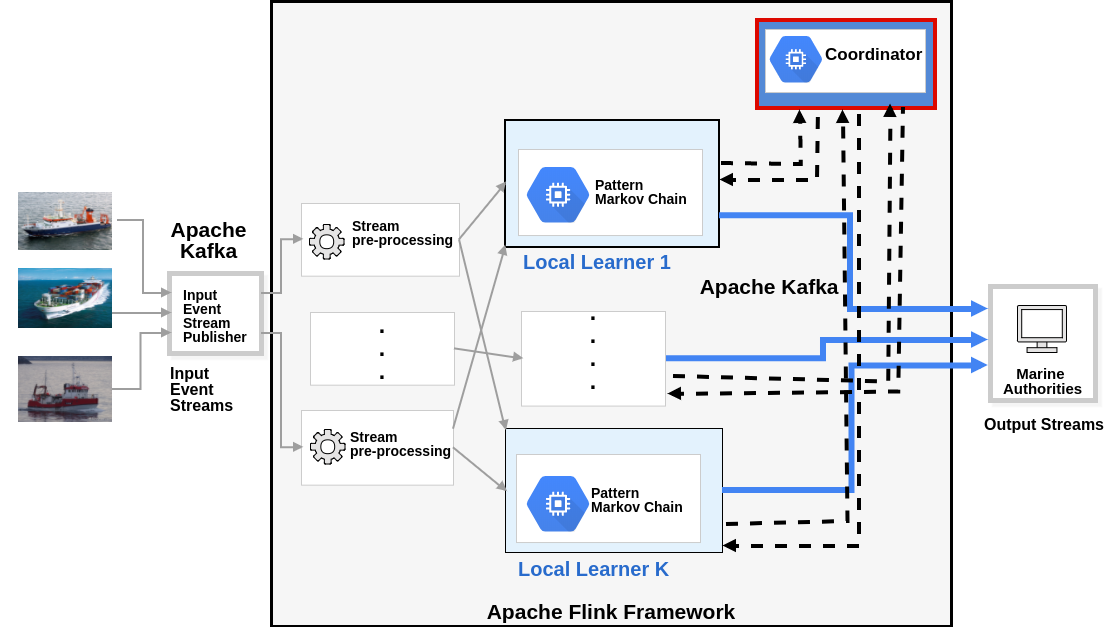
\includegraphics[height=2.5in, width=\linewidth]{figures/distributed_architecture.png}
	
\caption{System Architecture.}
\label{fig:architecture}
\end{figure}

The system is composed of three processing units:   \begin{enumerate*}[(i)]
	\item pre-processing operators that receive the input event stream, and perform filtration, ordering operations, before partitioned the input event stream to multiple event streams based on the associated moving object 
	\item predictor nodes (learners), which are responsible to maintain a prediction model for the input event streams, such that each prediction node is configured to handle an event stream from the same moving object, in order to provide online predictions for a predefined pattern $\mathcal{P}$  
	\item a coordinator node that communicates through a Kafka stream channels with the predictors to realize the distributed online learning protocol, which builds a global prediction model based on the received local models, and then share it among the predictors.
\end{enumerate*}

\par In summary, our distributed system consists of multiple pre-processing operators, prediction nodes,  and a central coordinator node. All units are running concurrently and arranged as data processing pipeline as depicted in Figure ~\ref{fig:architecture}. We leverage the Apache Kafka as messaging system to ingest the input event streams and to publish the result streams, in addition, it used as the communication channel between the predictor nodes and the coordinator. While Apache Flink is employed to execute the system's distributed processing units over the input event streams. Our system architecture can be modeled as logical network of processing nodes  organized in a Directed Acyclic Graph (DAG), which is inspired by the Flink runtime dataflow programs \cite{carbone2015apache}.  
